\subsection{Permissions}

\subsubsection{Users}
For our application we will have several users, spanning across multiple organizations. Many of these users will have vast amount of data that they will wish to keep secure if they are to use our application. The problem comes when the data that users have stored needs to become outward facing. Examples of this would be requests to pull files, accumulating data for our crowd sourced visualizations or showing snippets of interesting sound files to other users. In all, our application revolves around data and the visualization of that data. For this very reason we must be sure to keep user data secure and to have the trust of our users when implementing our ideas.\par
The very basis for our data security will stem from the use of Universally unique identifiers. These UUID\textquotesingle s are randomly generated 128 but numbers, that can be used to identify users. While collisions with this method are not zero, their occurrence is so seldom that checking is not required. Users will be assigned an identifier once they install the software and log-in. From that point forward all user activity will be tracked using the randomly assigned identifier and the user\textquotesingle s email, which will be required and authenticated to log in. Combining email and UUID provides an astronomically low chance of collisions. This will allow tracking of all user actions. Thus making sure that from the point of first use no creation or manipulation of data can be done without a user being connected to the action. This will allow for accountability to be held to an end user in case a malicious action is taken to destroy, obscure or otherwise harm data through our application.\par
By tracking all our users, we can then very easily set up permissions for each file or sets of files that are publicly facing through the application. Tables in our database will map files to the selected users that can see them. This will be cross-validated by also keeping track of what users can see the files. Both table entries must match for the file to be accessed by the requesting user.

\subsubsection{Groups}
Permissions may also be assigned to a set of users via groups. These groups will allow accumulations of users to share data together openly. The group will be controlled by an admin. This administrative position will have rights to add and delete users from the group. Along with the permission to move users around the admin may also set the shared access rights for the group. Certain individuals or organizations may want to allow access to groups of people. Instead of having to give permissions to each person, A user or organization may allow a set of users to see their data. This will allow for organizations, such as universities, to share with other organizations quickly. This will hopefully reduce the stress of having to remove and add new users as they cycle out of foreign organizations.

\begin{figure}[t]
  \begin{center}
  \captionsetup{width=.8\linewidth}
  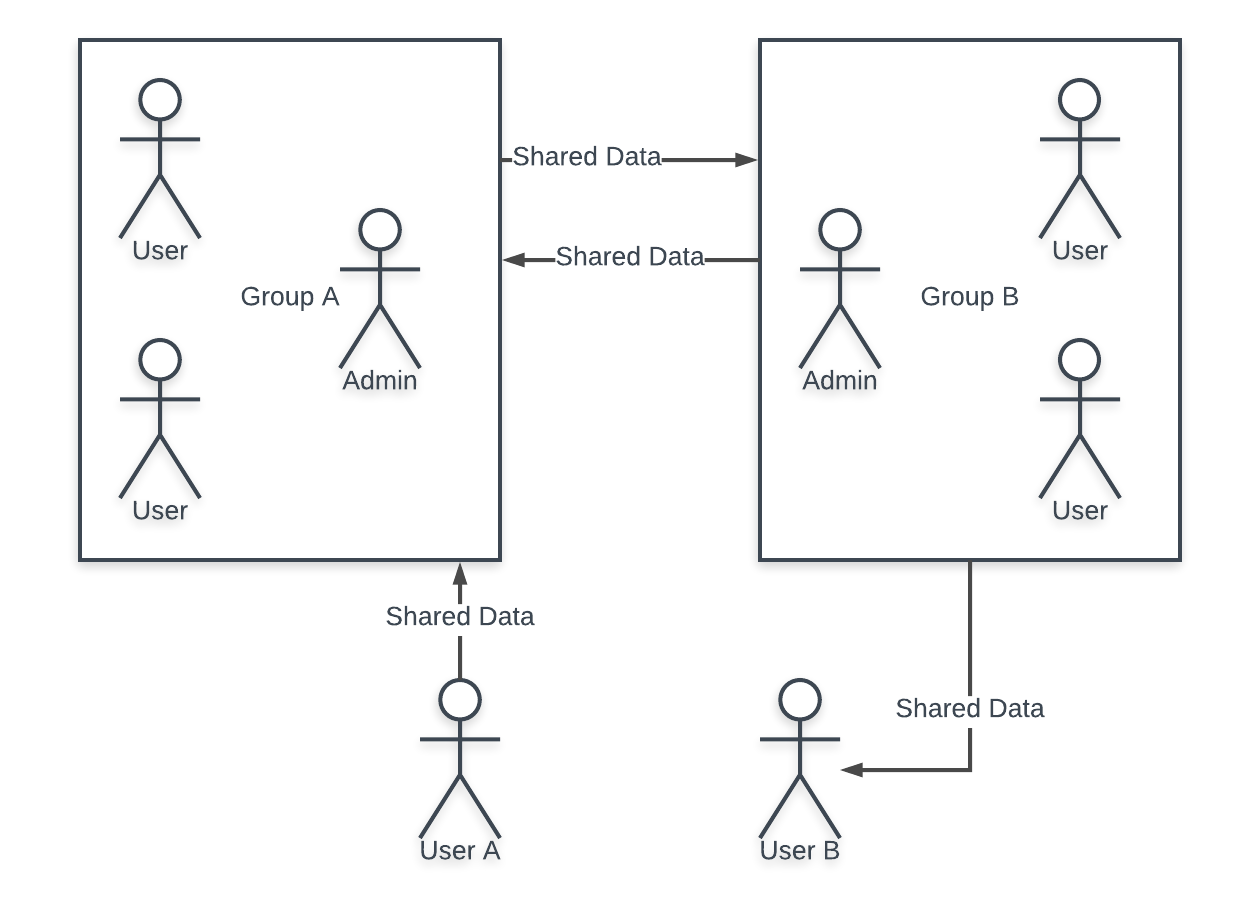
\includegraphics[width=0.8\linewidth]{DataPermissions}
  \caption{All users of Group A have permissions to User A's data; All Users from Group A have access to the data of Group B and vice versa; User B Has rights to Group B's Data; No group or user has access to User B's data}
  \end{center}
\end{figure}

\subsubsection{Access Rights}
Users and groups may set two types of access rights to their files. The first being open and the second being restricted. As the name states open files are open to the public. No special permission is needed to access them. Thus any user of our application may go to wherever they are hosted and pull them onto their own machine. If a user or group chooses that they do not wish to have their files/data open to the world then they may choose the restricted option. This option only allows certain users/groups to have access to the files/data. The specific rights are entailed below.\par
Users and groups may have different levels of permission given to them, refered to as access rights. These access rights can come in three forms. Right to read, right to edit, and right to pull. The right to read allows a users/groups to view the files/data the a user has published on the application. The right to edit allows users/groups to run analysis on data and use the tools we provide on the files/data. The right to pull allows users/groups to download the files/data from the hosts machine onto their local machine. From that point on whatever the local user does with the data is beyond the control of either us/ or anyone affiliated with our program.
